\documentclass{article}
\usepackage{amsmath, sfmath, multicol, tkz-euclide, array, enumerate, tcolorbox, tabularray}
\renewcommand{\familydefault}{\sfdefault}
\setlength{\parindent}{0cm}
\pagestyle{empty}
\usepackage[left=1in, top=0.5in, right=1in, bottom=0.5in]{geometry}
\tikzset{>=stealth}
\tcbset{colback=white}

\newcounter{example}[section]
\newenvironment{example}[1][]{\refstepcounter{example}\par\medskip
   {\color{red}\textbf{Example~\theexample. #1}}}{\medskip}

\begin{document}

\section*{Perimeter, Circumference, and Area}

\begin{tcolorbox}[colframe=orange!70!white, coltitle=black, title=\textbf{Today I Can}]
\begin{enumerate}
    \item Find the perimeter and circumference of basic shapes.
    \item Find the area of basic and composite shapes.
\end{enumerate}
\end{tcolorbox}

\begin{tcolorbox}[colframe=black!20!white, opacitybacktitle=0.1, coltitle=black, title=\textbf{Perimeter}]
The \textbf{perimeter} of a polygon is the sum of the lengths of its sides.
\end{tcolorbox}

\begin{tcolorbox}[colframe=black!20!white, opacitybacktitle=0.1, coltitle=black, title=\textbf{Area}]
The \textbf{area} of a shape is the number of square units it uses (i.e. how much space it takes up on paper).
\end{tcolorbox}

\vspace{0.25in}

\begin{tabular}{p{0.5\textwidth}p{0.4\textwidth}}
\textbf{Triangle}    &   \textbf{Square}  \\[15pt]
$\text{Area} = \frac{1}{2}bh$ &   $\text{Area} = s^2$   \\[10pt]
\raisebox{2.4cm}{
\begin{tikzpicture}
    \tkzDefPoints{0/0/A, 3/0/B, 1/2/C}
    \tkzDrawPolygon(A,B,C)
    \tkzLabelSegment[below](A,B){$b$}
    \tkzDefLine[orthogonal=through C](B,A) 
    \tkzGetPoint{D}
    \tkzInterLL(C,D)(A,B)
    \tkzGetPoint{E}
    \tkzDrawSegment[dashed](C,E)
    \tkzLabelSegment[below right](C,E){$h$}
\end{tikzpicture}}
&   \raisebox{2.4cm}{
\begin{tikzpicture}
    \tkzDefPoints{2/2/A, 4/2/B, 4/4/C, 2/4/D}
    \tkzDrawPolygon(A,B,C,D)
    \tkzLabelSegments[below](A,B){$s$}
    \tkzLabelSegments[right](B,C){$s$}
    \tkzMarkRightAngle(C,B,A)
\end{tikzpicture}}
\\[-2cm]
\textbf{Rectangle}   &   \textbf{Circle}    \\[10pt]
$\text{Area} = lw$    &   $\text{Area} = \pi r^2$; \quad $\text{Circumferene} = 2\pi r$   \\[10pt]
\raisebox{2.4cm}{
\begin{tikzpicture}
    \tkzDefPoints{0/0/A, 3/0/B, 3/2/C, 0/2/D}
    \tkzDrawPolygon(A,B,C,D)
    \tkzLabelSegments[below](A,B){$l$}
    \tkzLabelSegments[right](B,C){$w$}
    \tkzMarkRightAngle(C,B,A)
\end{tikzpicture}}
&
\raisebox{2.4cm}{
\begin{tikzpicture}
    \tkzDefPoints{0/0/A, 1.5/0/B}
    \tkzDrawCircle(A,B)
    \tkzDrawPoint(A)
    \tkzDrawSegment(A,B)
    \tkzLabelSegment[below](A,B){$r$}
\end{tikzpicture}}
\end{tabular}

\vspace{-0.5in}

\begin{example}
You want to frame a picture that is 5 in by 7 in with a 1-in wide frame.

\begin{multicols}{2}
\begin{enumerate}[(a)]
\item What is the area of the picture? 
\item What is the area of the frame? 
\end{enumerate}
\end{multicols}
\end{example}

\newpage 

\begin{example}
What is the perimeter and area of $\triangle EFG$ if $E(3, 6)$, $F(3, -2)$, $G(-3, -2)$? \newline\\

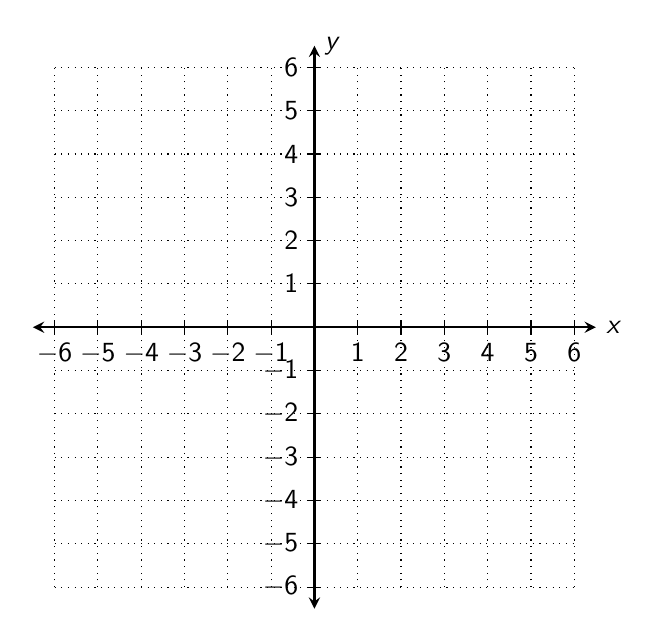
\begin{tikzpicture}[scale=0.55]
\draw[<->, thick] (-6.5,0) -- (6.5,0) node [right] {$x$};
\draw[<->, thick] (0,-6.5) -- (0,6.5) node [right] {$y$};
\draw[dotted] (-6,-6) grid (6,6);
\foreach \x in {-6,...,-1,,1,...,6}
\draw (\x, 0.15) -- (\x,-0.15) node [below] {$\tiny \x$};
\foreach \y in {-6,...,-1,,1,...,6}
\draw (0.15,\y) -- (-0.15,\y) node [left] {$\tiny \y$};
\end{tikzpicture}
\end{example}

\vspace{1in}

\begin{example}
What is the perimeter and area of each of the following?

\begin{enumerate}[(a)]
\begin{multicols}{2}
    \item \mbox{}
    \item \mbox{}
\end{multicols}
\end{enumerate}    
\begin{minipage}{0.5\textwidth}
\begin{tikzpicture}[scale = 0.7]
    \tkzDefPoints{0/0/A, 6/0/B, 6/2/C, 4/2/D, 4/4/E, 2/4/F, 2/6/G, 0/6/H}
    \tkzDrawPolygon(A,B,C,D,E,F,G,H)
    \tkzMarkSegments[mark = ||](A,H A,B)
    \tkzMarkSegments[mark = |](B,C C,D D,E E,F F,G G,H)
    \tkzLabelSegment[left,xshift=-0.1cm](H,A){9 cm}
    \tkzLabelSegment[above,yshift=0.1cm](H,G){3 cm}
    \tkzMarkRightAngles(A,B,C B,C,D C,D,E D,E,F E,F,G F,G,H G,H,A B,A,H)
\end{tikzpicture}
\end{minipage}
\begin{minipage}{0.4\textwidth}
    \begin{tikzpicture}
    \tkzDefPoints{0/1.5/F, 0/0/A, 4/0/B, 4/1.5/C, 1.5/1.5/E, 1.5/3/D}
    \tkzDrawPolygon(A,B,C,D,E,F)
    \tkzLabelSegment[below](A,B){12 ft}
    \tkzLabelSegment[left](F,A){4 ft}
    \tkzMarkSegments[mark = |](A,F F,E E,D B,C)
    \tkzMarkRightAngles(B,A,F C,B,A E,F,A D,E,F)
\end{tikzpicture}
\end{minipage}
% \begin{tabular}{p{0.6\textwidth}p{0.4\textwidth}}
% (a)     &   (b)     \\[0.1in]
% \begin{tikzpicture}[scale = 0.7]
%     \tkzDefPoints{0/0/A, 6/0/B, 6/2/C, 4/2/D, 4/4/E, 2/4/F, 2/6/G, 0/6/H}
%     \tkzDrawPolygon(A,B,C,D,E,F,G,H)
%     \tkzMarkSegments[mark = ||](A,H A,B)
%     \tkzMarkSegments[mark = |](B,C C,D D,E E,F F,G G,H)
%     \tkzLabelSegment[left,xshift=-0.1cm](H,A){9 cm}
%     \tkzLabelSegment[above,yshift=0.1cm](H,G){3 cm}
%     \tkzMarkRightAngles(A,B,C B,C,D C,D,E D,E,F E,F,G F,G,H G,H,A B,A,H)
% \end{tikzpicture}
% &
% \begin{tikzpicture}
%     \tkzDefPoints{0/1.5/F, 0/0/A, 4/0/B, 4/1.5/C, 1.5/1.5/E, 1.5/3/D}
%     \tkzDrawPolygon(A,B,C,D,E,F)
%     \tkzLabelSegment[below](A,B){12 ft}
%     \tkzLabelSegment[left](F,A){4 ft}
%     \tkzMarkSegments[mark = |](A,F F,E E,D B,C)
%     \tkzMarkRightAngles(B,A,F C,B,A E,F,A D,E,F)
% \end{tikzpicture}
% \end{tabular}
\end{example}

\end{document}
